\subsection{Trajectory Ontology}

Concepts in the \emph{Trajectory} module use the concepts from the Pollution ODP (Figure~\ref{fig:trajectory_concepts}). It models the trajectories of pollution carriers. For example, a wind current passing through a crop burning site may carry carbon based pollutants to another destination. This displacement of pollutants needs to be accounted for to get a holistic understanding of air pollution. The trajectory component has been adapted from the Trajectory ODP~\cite{10.1007/978-3-319-01790-7_24}. A brief description of the \emph{Trajectory} module concepts is as follows.

\begin{figure}[ht]
\centering
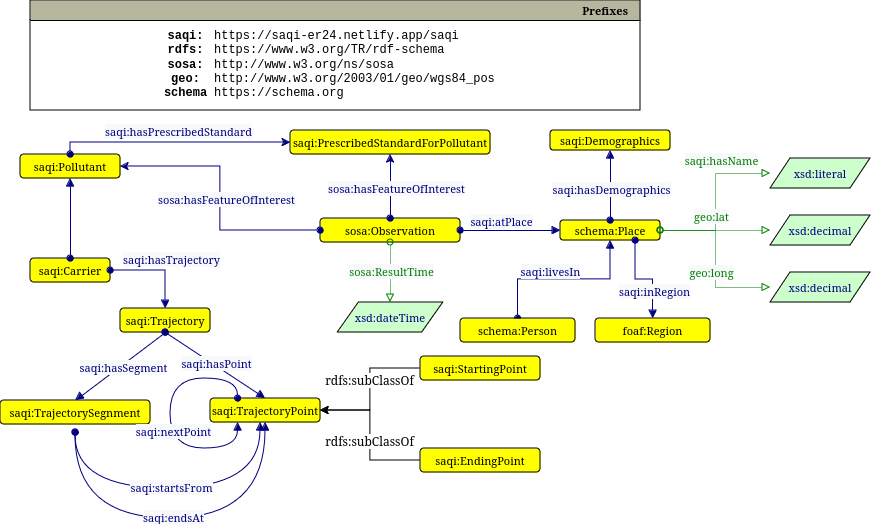
\includegraphics[height=6.5cm, width=0.90\textwidth]{figures/ObservationTrajectory.png}
\caption{Trajectory class and its connections} 
\label{fig:trajectory_concepts}
\end{figure}

\textbf{Trajectory.} The \texttt{Trajectory} concept represents a set of ordered spatiotemporal points. 

\textbf{TrajectoryPoint and TrajectorySegment.} The \texttt{Trajectory} concept is linked to the \texttt{TrajectoryPoint} and \texttt{TrajectorySegment} through the \texttt{hasPoint} and \texttt{hasSegment} properties. The \texttt{nextPoint} property links trajectory points in the
appropriate order within a trajectory. The segments in the trajectory are defined by a starting trajectory point \{$x_i$, $y_i$, $t_i$\} and an ending trajectory point \{$x_j$, $y_j$, $t_j$\} where $t_i$, $t_j$ denote time points such that $t_i$ $<$ $t_j$ . The \texttt{TrajectorySegment} concept represents this notion of a segment which is connected to two fixes through \texttt{startsFrom} and \texttt{endsAt} properties.

%\begin{figure}[ht]
%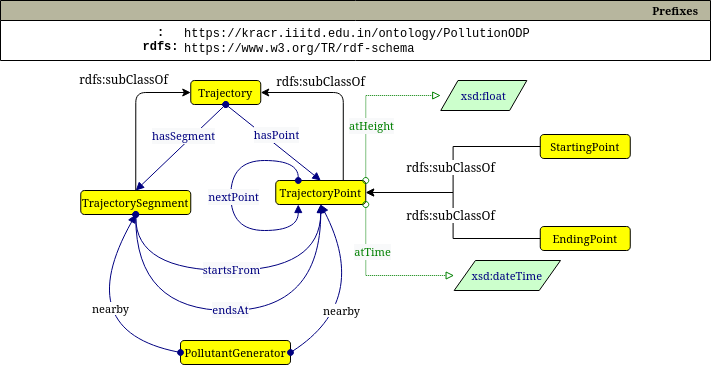
\includegraphics[ height=4.5cm]{figures/Trajectory.png}
%\caption{Trajectory concepts in PollutionODP} 
%\label{fig1}
%\end{figure}